%%%%%%%%%%%%%%%%%%%%%%%%%%%%%%%%%%%%%%%%%%%%%%%%%%%%%%%%%%%%%%%%%%%%%%%%
% Copyright (c) 2022 Antonio Coín
%
% This work is licensed under a
% Creative Commons Attribution-ShareAlike 4.0 International License.
%
% You should have received a copy of the license along with this
% work. If not, see <http://creativecommons.org/licenses/by-sa/4.0/>.
%%%%%%%%%%%%%%%%%%%%%%%%%%%%%%%%%%%%%%%%%%%%%%%%%%%%%%%%%%%%%%%%%%%%%%%%

%%%%%%%%%%%%%%%%%%%%%%%%%%%%%%%%%%%%%%%%%%%%%%%%%%%%%%%%%%%%%%%%%%%%%%%%
\chapter{Model choice, implementation and validation}\label{ch:model-choice}
%%%%%%%%%%%%%%%%%%%%%%%%%%%%%%%%%%%%%%%%%%%%%%%%%%%%%%%%%%%%%%%%%%%%%%%%
In this section we gather together several remarks on the main choices made throughout the design of our model, as well as some validation strategies that attempt to measure the goodness-of-fit of the model given the observed data.

\paragraph{The choice of \(\symbf p\).} One of the key decisions in our Bayesian modeling scheme was whether to consider the number of components \(p\) as a member of the parameter space and integrate it into the model. While theoretically we could impose a prior distribution on \(p\) as well (e.g. a categorical distribution with a fixed maximum value), we found that it would have some unwanted practical implications. For instance, it would make the implementation more complex, since the dimensionality of the parameters \(b\) and \(\tau\) would need to be fixed at a certain maximum value beforehand, but the working value of \(p\) within the MCMC algorithm would vary from one iteration to the next. In this case we would face a label switching issue \citep[c.f.][Sec.~2.3]{grollemund2019bayesian}, as we would have no way of knowing which set of parameters is ``active'' at any given time. Another possibility would be to adapt a purely Bayesian model selection technique \citep[e.g.][Ch.~7]{piironen2017comparison, gelman2013bayesian} to our framework, or even derive some model aggregation methods to combine the posterior distributions obtained for different-sized models. In the end, for the sake of simplicity we decided to let \(p\) be an hyperparameter, so that we could use any model selection criteria (e.g. BIC, DIC, cross-validation, \ldots) to select its optimal value. This is equivalent to imposing a degenerate prior distribution on \(p\). Moreover, the experiments carried out indicate that even low values of \(p\) provide sufficient flexibility in most scenarios (see Section~\ref{sec:results}). \incomment{Reversible MCMC}

%Reversible-jump MCMC
% Estos métodos permiten variar la dimensionalidad subyacente del espacio muestral en cada propuesta (\sidecite[*0]{green1995reversible}). Teóricamente son útiles para muestrear de mixturas de gaussianas, procesos de Dirichlet o, en general, de cualquier distribución donde haya una variable latente que represente la dimensión del espacio. Sin embargo, no hay una implementación de referencia establecida.

\begin{outcomment}
Reescribir label switching (nos pasa; lo que pasa que con p free se acentua).

Ocurre porque el likelihood es simetrico: L(theta mid y) = L(thetaperm mid y) para cualquier permutacion (hay p! posibles) --> no-identificabilidad.

"In these situations, parameter estimates and other output are inevitably aggregated
across numerous replications, and because the labels of the enumerated classes are
arbitrarily assigned, there is no guarantee that the same class would have the same
label from replication to replication."

From a Bayesian pointof view, this amounts to truncating the original prior distribution... (to verify the constraints)

As a result, in any MCMC algorithm, labels of the
components can permute multiple times between iterations of the sampler.
Paradoxically, as noted by Celeux, Hurn and Robert (2000), Fruhwirth-Schnatter (2001),
Jasra, Holmes and Stephens (2005) and Papastamoulis and Iliopoulos (2010), among others,
label switching is a prerequisite for MCMC convergence. If there is no label switching it
means that the sampler is not exploring all the modes of the posterior distribution of (1)

"When sampling from the unconstrained posterior via MCMC methods, which component of the sampled parameter corresponds to which state is unknown due to potential label switching." Si usamos la marginal para haacer inferencia --> nonsensical answers (Stephens, 2000)

Solución: añadir constraints de identificabilidad artificiales (ej relabeling, mantener ordenados, posprocesado).

Imposing an identifiability constraint on the parameters breaks the sym-
metry of the posterior distribution of the parameters, and so we might hope that it would allow us to perform sensible inference for the individual components of the mixture. Inference conditional on such a constraint may be performed by post-processing the sample (proposition 3.1 in Stephens 1997 phD thesis).

OTRA OPCION: Elegir en cada iteración como parámetro para ordenar aquel que deja mayor separación (tras escalarlos todos a [0,1]): \verb@https://helda.helsinki.fi/bitstream/handle/10138/329485/Approximate_Bayesian_computation_for_finite_mixture_models.pdf?sequence=1@

OTRA SOLUCION: "Adaptive Metropolis with Online Relabeling" --> The key step is the selection, after each proposal of a permutation (relabeling) of the proposed vector by minimizing a quadratic cost function
$L_{t-1} (x)$ over all permutations of the proposed vector, where L is defined by
$L_t(x) = (x - \mu)'\Sigma^{-1}(x - \mu)$
This step forces the posterior sample to look as unimodal as possible.

Citas: Stephens (2000), Papastamoulis \& Iliopoulos, 2010; Rodriguez \& Walker, 2014
\end{outcomment}

Aunque se puede tener en cuenta solo las primeras 'p' posiciones, en el propio algoritmo de MCMC no se puede 'apagar' fácilmente el valor de los betas que no se usan, por lo que crecen indefinidamente y generan problemas (lo mismo ocurre con los 'tau', que incluso se pueden salir de rango). Aunque una posible solución es limitar todos los taus y no solo los p primeros, esto solo retrasa el problema (con cadenas más largas vuelve a ocurrir, además de ocasionar el problema "RuntimeWarning:covariance is not positive-semidefinite." con el WalkMove), ya que los betas no están limitados. Podríamos intentar limitarlos a un valor razonable.

Por otro lado, en algunas cadenas el sigma2 es más grande de la cuenta, ya que tiende a "compensar" la falta de flexibilidad del modelo (e.j. si el valor de p es más bajo). Esto hace que los estimadores basados en la media y en el posterior mean sean ligeramente peores (sobre todo el de la media puntual, donde la varianza estimada sí se ve notablemente afectada). Quizás para contrarrestar esto habría que tener un modelo con un $\sigma^2_p$ para cada valor de p?

Además, aunque todo esto funcionase, si por ejemplo en una iteración el modelo elige p=2, está optimizando beta1 y beta2 para ese caso; si luego miramos solo la marginal de beta1, se habrán mezclado los casos en los que p=1 y beta1 debe valer una cosa, y en los que p=2 y beta1 vale otra cosa potencialmente distinta (se puede compensar con beta2, hay más grados de libertad).

\paragraph{Other hyperparameters.} As for the default values of the rest of hyperparameters in~\eqref{eq:prior-linear}, several comments are in order:
\begin{itemize}
  \item For the expected value \(b_0\) we propose to use the MLE of \(b\). Although the likelihood function is rather involved, an approximation of the optimal value is enough for our purposes (see Section~\ref{sec:results} for details on the implementation). Our numerical studies suggest that the results are much better with this choice than, say, with a random or null vector.
  \item We found that the parameter \(g\) does not have as much influence on the final result, and the experimentation suggests that \(g=5\) is a good value.
  \item Lastly, we observed that the choice of \(\eta\) can have a considerable impact on the final estimator. That is why, in an effort to normalize its scale, we consider a compound parameter \(\eta = \tilde \eta \lambda_{\max}(\mathcal X_\tau'\mathcal X_\tau)\), where \(\lambda_{\max}(\mathcal X_\tau'\mathcal X_\tau)\) is the largest eigenvalue of the matrix \(\mathcal X_\tau'\mathcal X_\tau\), and \(\tilde\eta > 0\) is the actual tuning parameter. This standardization technique has been used previously in the literature; see for example \citet{grollemund2019bayesian}.
\end{itemize}

\paragraph{Summarizing the posterior.} On a separate note, observe that the choice of a specific point estimator to summarize the posterior distribution results in a veiled assumption of an underlying loss function between the estimated and real parameters. In general, the mean is more sensitive to outliers and the median is more robust, but the latter assumes an \(L^1\)-type loss function while the former implicitly optimizes an \(L^2\) loss. On the other hand, the mode is also a good candidate because it represents the point of highest probability density. At any rate, these decisions are strongly dependent on several factors such as the skewness or the number of modes in the resulting posterior distribution, and thus should be made on a case-by-case basis. \incomment{Argue that, because of the label switching and multimodality, summarizing the posterior might be impractical, unhelpful, misleading, etc. So the best strategy is the posterior mean.}


\begin{outcomment}
  Sección para elección del algoritmo mcmc. Contar que también se usa pymc (PPL, probabilistic programming language) y que en particular se probaron metropolis y NUTS: "Dentro de estos métodos destaca el \textit{No U-Turn Sampler} (NUTS, \citet{hoffman2014no}), que tiene la ventaja añadida de que realiza un ajuste automático de hiperparámetros."

  % Otra de las ventajas que ofrece este método frente a algoritmos clásicos es que solo requiere fijar unos pocos hiperparámetros (independientes de la dimensión subyacente), en lugar de los \(O(N^2)\) correspondientes, por ejemplo, a la matriz de covarianza de la distribución de salto \(N\)-dimensional en Metropolis-Hastings. Además, el paquete ha sido extendido para admitir otro tipo de movimientos paralelos, y el objetivo del proyecto es proporcionar un método de muestreo de propósito general que funcione correctamente en una clase amplia de problemas. Es muy usado por ejemplo en el campo de la astrofísica, y está bien establecido y testeado.
\end{outcomment}

\begin{outcomment}
  Sección para inicialización.

  También en el artículo citado se aconseja inicializar las cadenas en una bola gaussiana alrededor de un punto que se espere que tenga alta probabilidad según \(p(x)\).
\end{outcomment}


\paragraph{Model validation and Bayesian checks.} To conclude, it is worth mentioning that the Bayesian aspects of our model allow us to perform some model validation checks straight away. For example, we can derive credible intervals for each of the parameters, and in the case of linear regression, we can use the sampled values of \(\sigma^2\) as a measure of the uncertainty of the predictions. Moreover, we can perform various \textit{visual checks}, such as a plot comparing both the observed and posterior predictive distribution of the responses, or a diagram showing the distribution of some statistic \(T(\symbf Y^*)\) of the posterior predictive distribution \(\symbf Y^* \equiv \{\symbf Y^{(m)*}\}\) (see Figure~\ref{fig:ppc}). In addition, we can calculate the so-called \textit{Bayesian p-values} for several statistics, which are defined as \(P(T(\symbf Y^*)\leq T(\symbf Y)| \symbf Y)\), and are computed by simply measuring the proportion of the \(M\) approximate estimates \(T\{\symbf Y^{(m)*}\}\) that fall below the real value of the statistic. They are expected to be around 0.5 when the model accurately represents the data, and a deviation either way can be indicative of modeling issues; see Chapter 6 of \citet{gelman2013bayesian} for details.

\begin{figure}[ht]
  \centering
  %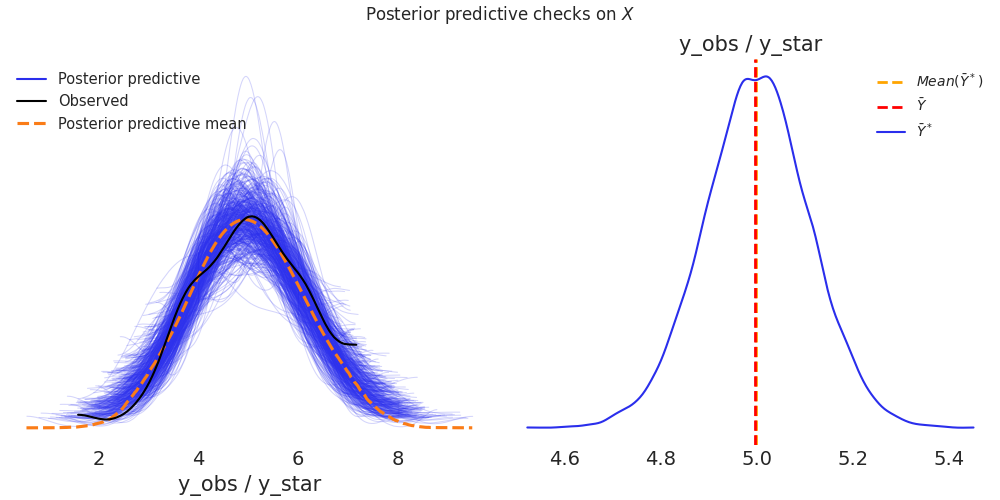
\includegraphics[width=.75\textwidth]{img/ppc_linear}
  \caption{Posterior predictive graphical checks on a fitted model. On the left there is a comparison between the observed distribution of the response variable and the posterior predictive distribution of the approximate sampled responses, while the distribution of the average of the posterior predictive responses is depicted on the right.}\label{fig:ppc}
\end{figure}
